\documentclass[11pt, letterpaper]{article}
\usepackage[margin=1in]{geometry}
\usepackage[small]{titlesec}
\usepackage{indentfirst}
\usepackage{graphicx}
%opening
\title{\vspace{-2.5cm}Monet-Style GAN Art Generator}

\author{Austin Gardiner and Seth Dana}
\date{STAT 6685}

\begin{document}

\maketitle


\section*{Goals and Data}
The goal of this project is to create a generative adversarial network (GAN) capable of generating Monet-style artwork from a photo input. This project idea came from Kaggle and is part of a competition titled “I’m Something of a Painter Myself”. This GAN will be made up of a generator and discriminator model. Since the GAN is generating data and not being told what the output should look like through labels, this is considered an unsupervised learning problem. The discriminator model works with supervised learning as it is given two possible labels, real or generated. The model learns through an adversarial training process. \\

The training data consists of paintings by Monet and photos in a 256x256 JPEG format. Kaggle provides 300 Monet paintings and 7028 photos. If our discriminator model needs more true Monet paintings, we can mirror the 300 paintings we have to give us 600. We assume that the style of the painting will be preserved even if the painting is mirrored. Initially our models will only use the 300 Monet paintings and 7028 photos, but data augmentation will be tested to see if the model improves. 

\begin{figure}[h] % replace 't' with 'b' to force it to be on the bottom
	\centering
	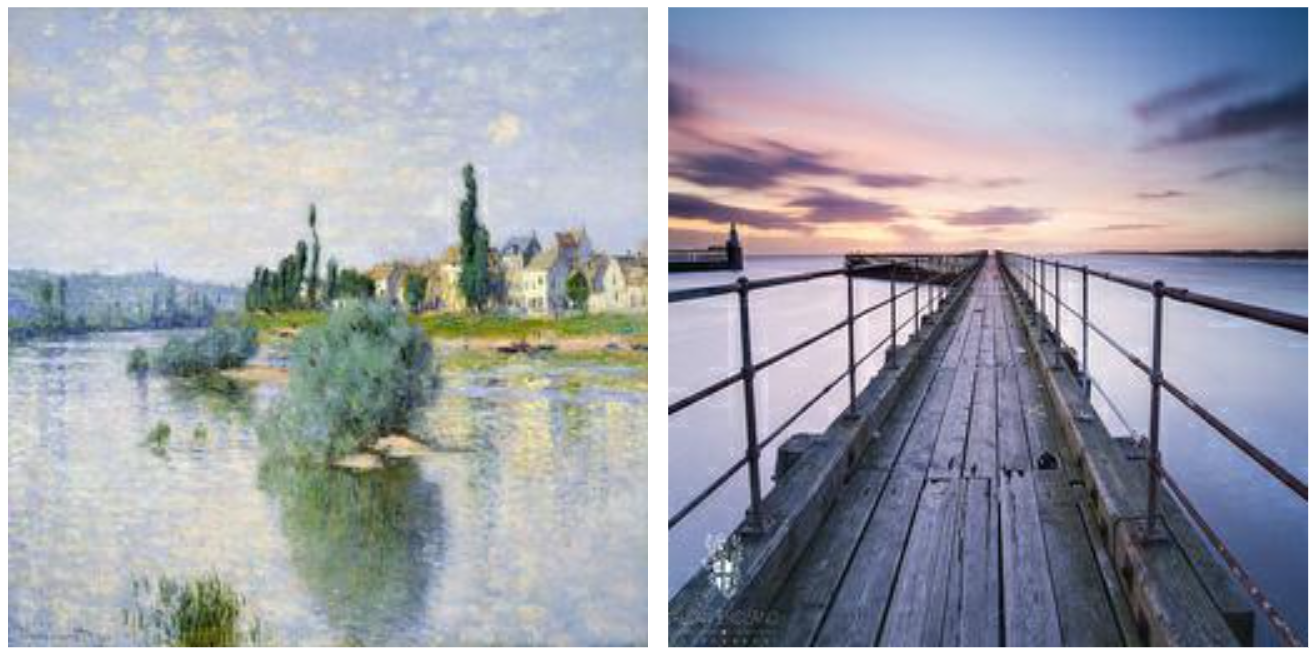
\includegraphics[width=0.6\textwidth]{data.png}
	\caption{A Monet painting and photo example from the training data.}
\end{figure}   

\section*{Methods}
A generative adversarial network consists of two competing models, a generator and a discriminator. In the case of our project, the generator takes jpeg images as inputs and transforms them into Monet-style paintings. The discriminator is a binary classifier whose goal is to classify the transformed outputs from the generator as being real Monet paintings or as generated fakes. The adversarial training process describes the cycle where a better generator is able to trick the discriminator more often and as the discriminator gets better, it is more accurate in distinguishing our generated images from true Monet paintings. \\

Our plan is to use convolutional neural networks (CNN) for both the generator and the discriminator models. Both will use transfer learning from pre-trained CNN models that will be further trained on the provided set of Monet paintings. The generator will use a series of convolutional layers, pooling layers, and skip connections to unpooling and deconvolution layers. The discriminator will also use convolutional layers and pooling layers, but will then feed into fully connected layers to get the binary classification output. \\

Because the GAN consists of two neural networks, for our baseline testing we will focus our comparisons on the discriminator performance with respect to basic machine learning methods. Because this is a binary classification task, we plan to test the discriminator against a Random Forest model, a Support Vector Machine model, and a K Nearest Neighbors model. In our research we found the suggestion of using some simple filter-based methods like histogram matching for style transfer and will attempt this for the generator.

\section*{Potential Issues}
One of the main problems we expect to run into is a lack of non-CNN based style transfer models. Almost all style transfer methods that we have found involve the use of CNNs, so we do not expect to have a good non-neural network option to compare the generator to. Also, with a GAN, we will have to train and tune two models. This will require extra time and effort. Last, we only have 300 Monet paintings in the dataset, which is not a lot to train on. We will try some data augmentation techniques and will use pre-trained CNN models to hopefully combat this challenge.

\section*{Project Management}
\begin{enumerate}
	\item Create GAN structure
	\item Create the CNN generator
	\item Create the CNN discriminator
	\item Create the ML discriminator
	\item Training and hyperparameter tuning
		\begin{itemize}
			\item[a.] Train and tune the generator
			\item [b.] Train and tune the discriminators
		\end{itemize}
	\item Compare results
\end{enumerate}

Both team members will work together to create the GAN structure and create the basic implementation of the generator and discriminators. It is expected that the generator and CNN discriminator will take roughly the same amount of time to implement, with the discriminator being slightly quicker to implement. As such, our plan is to have one team member focus on the generator, while the other focuses on the discriminators. \\

Once the structure and basic implementations are done, the team members will continue to work on tuning and training the generator and discriminators. The team member in charge of the generator will tune and train the generator, and the team member in charge of the discriminators will tune and train the discriminators. With both models completed, the team members will work together to compare the results. All reports will be written by both team members.



\end{document}
